\section{Peformance Evaluation}

\label{sec:evaluation}

\begin{figure}[ht] 
\centering
\subfigure[{}]{ 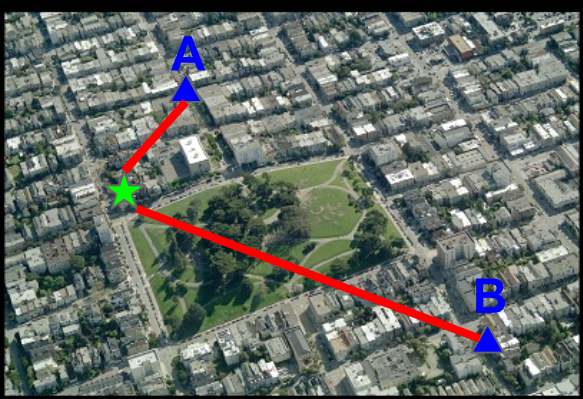
\includegraphics[width=0.3\textwidth]{pictures/eval-a} \label{eval-a} }
\subfigure[{}]{ 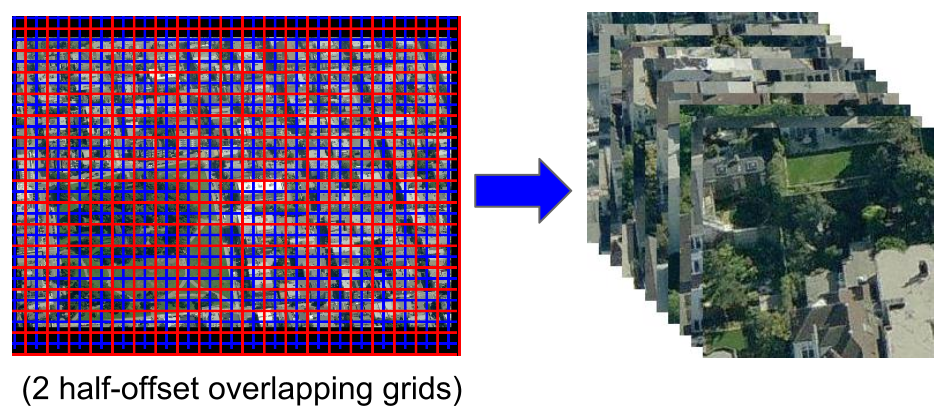
\includegraphics[width=0.5\textwidth]{pictures/eval-b} \label{eval-b} }
\caption[]{\subref{eval-a} Euclidean distance from a query (star) to a candidate location (A or B) is an unsatisfactory performance metric. \subref{eval-b} In our study we break the aerial views into blocks and use the rank of the true block as a performance metric.}
\label{eval}
\end{figure}


The evaluation on this dataset is done by first cutting the aerial image into overlapping blocks of size $200 \times 200$ pixels. Then the algorithm is asked to sort the blocks based on their matching scores. After that, the rank of the correct block is a used as a measure to compare different algorithms. Since the blocks are sorted based on matching score, it is desired for the correct block to have a low rank. We propose this measure because the traditional distance measures (e.g., Euclidean or geodesic) are not meaningful in this setting; see Fig.\ref{eval}\subref{eval-b}.  In the case of large search spaces, as in the IM2GPS setting, such a distance measure can reveal the neighborhoods in an entire country that have a similar visual texture to a query image.  In our setting, we only aim to find the genuine location such that user can verify the exact matched block. Therefore, we do not reward the matching if it misses the correct location but finds a non overlapping nearby location.

%we do not want to reward the matching algorithm if it misses the correct location but finds another location in the same city.

%The evaluation on this dataset is done by first cutting the aerial image into overlapping blocks of size $200 \times 200$ pixels. Then the algorithm is asked to sort the blocks based on their matching scores. After that, the rank of the correct block is a used as a measure to compare different algorithms. Since the blocks are sorted based on their matching scores, it is desired for the correct block to have a low rank. This measure is designed because the traditional distance measures are not meaningful for this purpose. For example, Euclidean spatial distance between the correct location and output of the algorithm is not a meaningful measure because if the algorithm does not discover the genuine location, it does not matter if the output is very far or rather close. This is true when the search is done within a small neighborhood, but if the search space was larger to cover different cities, finding the correct city is not far from being possible because of the correlation between the appearance of the buildings in the same city. Then in that case the spatial distance will be more meaningful. But in GLAID since there is no correlation between adjacent buildings, finding a wrong but close location should not be rewarded. This can be seen in Fig.\ref{eval}\subref{eval-b}, in which Point A is not preferred to B because of its shorter distance to the correct location. 
%[[I sense that this observation will be considered controversial by some reviewers, 
%  Mohammad: I changed the paragraph a little bit, it may be better. What do you think? Should we remove this observation?  Serge: yes, this is better.]]





%This dataset will be available for public use on UCSD Vision Group's Website \footnote{http://vision.ucsd.edu/}.
%This dataset will be available for public use on our group's website\footnote{link is removed for anonymity}.
